% zip -r graphical-inference.zip *.pdf *.tex images references.bib *.cls

% 8 pages, including reference 
% 
% Frame as design paper:
% 
%   * explain the target problem
%   * enough background that the reader can pass judgement about whether your
%     solution is good
%   * you should present results that back up the claim that your approach is
%     better than others
%
% Supplemental material to create plots
\documentclass[journal]{vgtc}
\usepackage{mathptmx}
\usepackage{graphicx}
\graphicspath{{plots/}}
\usepackage{times}
\usepackage{booktabs}
\usepackage[utf8]{inputenc}
\usepackage[square,sort&compress]{natbib}

\usepackage{tikz}
\definecolor{female}{HTML}{EF8A62}
\definecolor{male}{HTML}{67A9CF}
\definecolor{not-too-happy}{HTML}{FC8D59}
\definecolor{pretty-happy}{HTML}{FFFFBF}
\definecolor{very-happy}{HTML}{91CF60}
\definecolor{grey30}{HTML}{4D4D4D}
\newcommand{\key}[1]
  {\protect \tikz{\fill[#1] rectangle (1ex,1ex);}}


\onlineid{0}
\vgtccategory{Research}
\vgtcinsertpkg

\title{Product plots}
\author{Hadley Wickham, and Heike Hofmann}
\authorfooter{
  \item Hadley Wickham is an Assistant Professor of Statistics at Rice University, Email: hadley@rice.edu.
  \item Heike Hofmann is an Associate Professor of Statistics at Iowa State University.
}
\shortauthortitle{Wickham \MakeLowercase{\textit{et al.}}: Product plots}

\abstract{We propose a new framework for visualising counts or proportions, including existing graphics such as bar charts, mosaic plots, treemaps, equal area plots and fluctuation diagrams. We call our framework product plots, alluding to the computation of area as a product of height and width, and the statistical concept of generating a joint distribution from the product of conditional and marginal distributions.}

\keywords{Statistics, joint distribution, conditional distribution, treemap, bar chart, mosaic plot}
\CCScatlist{ % not used in journal version
  \category{H.5.2}{Information Interfaces and Presentation}{ User Interfaces --- Graphical user interfaces (GUI), Interaction styles, Screen design, Evaluation/methodology}
  \CCScat{I.6.8}{Computing Methodologies}%
  {Simulation and Modeling}{Visual Simulation};
}

% \teaser{
% \centering
% \includegraphics[width=16cm]{tx-cancer}
% \caption{One of these plots doesn't belong. These six plots show choropleth maps of cancer deaths in Texas, where darker colors = more deaths. Can you spot which of the six plots is made from a real dataset and not simulated under the null hypothesis of spatial independence?  If so, you've provided formal statistical evidence that deaths from cancer have spatial dependence. See Section~\ref{sec:solutions} for the answer.}
% \label{fig:teaser}
% }

\renewcommand{\manuscriptnotetxt}{\itshape Manuscript received 31 March 2011; accepted XX XXXX XXXX; posted online XX XXXX XXXX; mailed on XX XXXX XXXX. 

For information on obtaining reprints of this article, please send email to: tvcg@computer.org.}


\begin{document}
\firstsection{Introduction}
\maketitle

Tables of counts or proportions are an extremely common form of data. Correspondingly, there are many visualisations to display them. In this paper, we develop a framework that encompasses many existing visualisations, from bar charts to treemaps to pie charts, showing how graphics that previously seemed unrelated in fact share a deep underlying connection, and providing a systematic foundation for the developing new types of count visualisations \citep{cox:1978}.

Our framework focusses on area charts, where the area of a graphical element is proportional to the underlying count. We call our framework product plots in allusion to two products: the product of width and height to compute area, and the product of conditional and marginal distributions to produce joint distributions. A key development of our framework is the inverse operation: the factorisation of area plots. This allows easy extension from low-dimensional graphical primitives to high-dimensional data sets.

Section~\ref{sec:primitives} we motivate the three constraints that give rise to the fundamental graphical component of productplots: the rectangle. The rectangle gives rises to three fundamental 1d atoms (bar, spine, tile) and one fundamental 2d atom (the fluct). These constraints will later be relaxed in Section~\ref{sec:variations} to extend our framework to include even more visualisations including histograms, pie charts, cascaded treemaps and weighted plots.

Section~\ref{sec:combination} provides the mathematical framework that extends the simple 1d and 2d atoms to display data of any dimensionality, by showing just as any high dimensional joint distribution can be represented as a product of low-dimensional conditional and marginal distributions, any area plot can be decomposed into products of simple low-d primitives. Using this framework, Section~\ref{sec:existing} shows how 13 existing named graphics are just special cases of this general pattern.

To illustrate these ideas, we will use the same data for all examples. The data is a small sample of variables related to happiness from the general social survey ({\sc gss}) \citep{davis:2008}. The {\sc gss} is a yearly cross-sectional survey of Americans, run from 1976. We combine data for 25 years to gives 51\,020 observations, and of the over 5\,000 variables, we select eight related to happiness, as described in Table~\ref{tbl:happy}.

\begin{table*}[htb]
  \begin{center}
  \begin{tabular}{llp{9cm}}
    \toprule
    Variable & Description & Values \\
    \midrule
    {\sf age} & age in years & 18--89 \\
    {\sf degree} & highest education & lt high school, high school, junior college, bachelor, graduate \\
    {\sf finrela} & relative financial status & far above, above average, average, below average, far below \\
    {\sf happy} & happiness & \key{very-happy} very happy, \key{pretty-happy} pretty happy, \key{not-too-happy} not too happy \\
    {\sf health} & health & excellent, good, fair, poor \\
    {\sf sex} & sex & \key{female} female, \key{male} male\\
    {\sf wtsall} & probability weight & 0.43--6.42 \\
    {\sf year} & year of survey & 1972--2006 \\
    \bottomrule
  \end{tabular}
  \end{center}
  \caption{Description of sample data. Common plot colours are shown next to respective levels.}
  \label{tbl:happy}
\end{table*}

\section{Graphical primitives}
\label{sec:primitives}

All area plots correspond to tilings of the plane. We could consider partitions of higher-d spaces (e.g. 3d or 4d), but given that we have to project these down to 2d for viewing on paper or screen, there is little disadvantage to working directly in 2d. There are many possible ways to tile the plane. To weed these down to a manageable number, we identify three constraints \citep{keim:2002} important for visualising counts:

\begin{itemize}

  \item Area must be {\bf proportional} to count. Because the total area for a graphic is usually constrained, and area plot partitions the total, area plots display proportions, not counts. From here on, without loss of generality, we will refer to visualisation of proportions, rather than counts.

  \item Partitions must be {\bf rectangular}, because rectangles are easier to compare than arbitrary polygons \citep{cleveland:1984,cleveland:1986,heer:2010}, and are recursive in the sense that we can always tile a rectangle with smaller rectangles. This is not true for most shapes.

  \item Partitions must be {\bf disjoint}. To be able to see the complete area, each rectangle must be non-overlapping. This does not imply that the tiling must be space-filling.

\end{itemize}

\noindent Each of three constraints can be profitably relaxed, as detailed in Section~\ref{sec:variations}.

These constraints give rise to four graphical primitives. Section~\ref{sub:part-1d} describes the partitions of 1d data, bars, spines and tiles, and Section~\ref{sub:part-2d} describes the one partition of 2d data, the fluct.

% Let $a(i)$ give the area assigned to category $i$, which has proportion $f(i)$. Since we are using rectangles, $a(i) = k \dot a(i) = k \dot w(i) \times h(i)$ where $w$ and $h$ represent width and height respectively. Certain partitions also satisfy the constraint that $h(i) = \sqrt{k} f(i)^x$ and $w(i) = \sqrt{k} f(i)^y$ where $x + y = 1$. This is useful because it is only necessary to inspect one border to compare magnitudes.

\subsection{1d primitives}
\label{sub:part-1d}

1d primitives display one dimensional proportion data, i.e.\ proportions broken down by a single variable. There are three 1d primitives, as shown in Figure~\ref{fig:part-1d}. 

\begin{figure}[htbp]
  \centering
  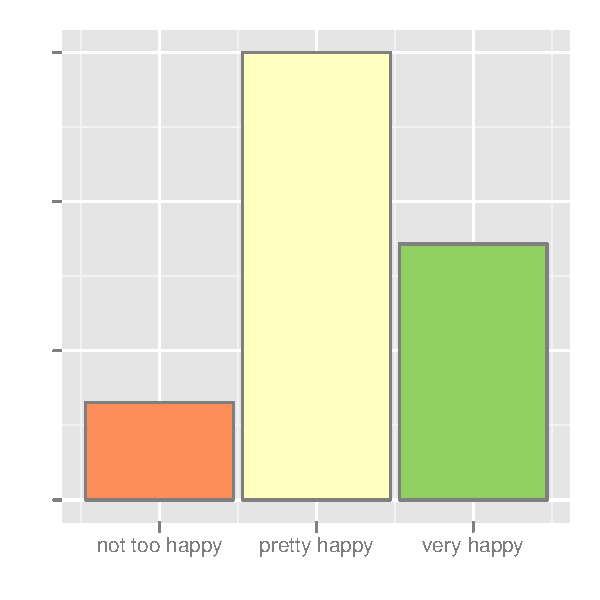
\includegraphics[width=0.33\linewidth]{part-hbar}%
  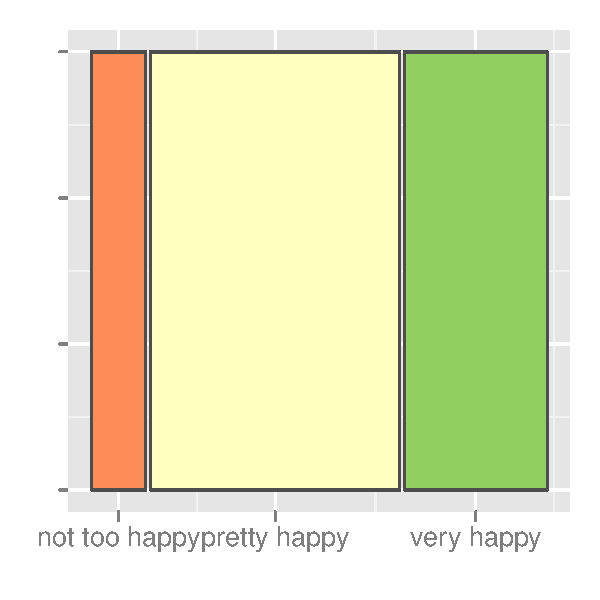
\includegraphics[width=0.33\linewidth]{part-hspine}%
  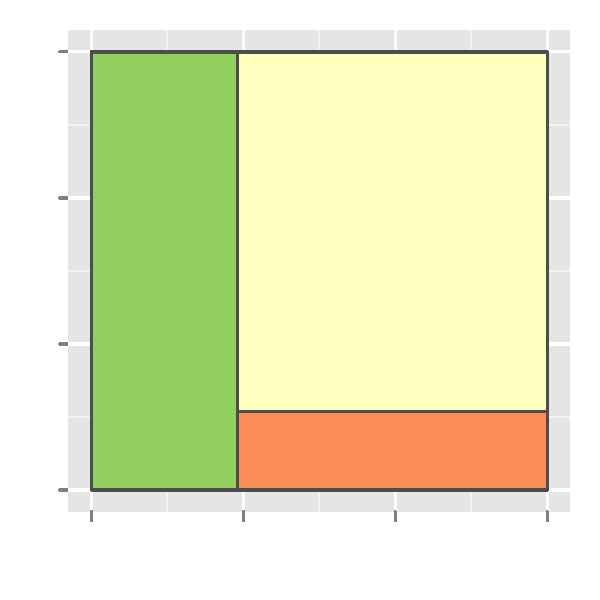
\includegraphics[width=0.33\linewidth]{part-treemap}

  \caption{1d partitions showing the distribution of happiness.  From left to right: bars, spines and tiles.}
  \label{fig:part-1d}
\end{figure}

\begin{itemize}
   \setlength{\itemsep}{0em}

  \item {\bf bar}s: height is proportional to value, width equally divides space. Bars are not space filling, occupying $\mbox{mean}(x - \max(x))$ of the total area. Bars can be arranged horizontally (``hbar'') or vertically (``vbar'').

  \item {\bf spine}s: width is proportional to value, height occupies full range. Spines are space filling and can be arranged horizontally (``hspine''), vertically (``vspine''), or can automatically pick their orientation (``spine'') by splitting the largest dimension. The name spine is evocative of books sitting on a library shelf \citep{hummel:1996}. Bars and spines are identical when visualising uniformly distributed data.

  \item {\bf tile}s: no restrictions on height or width, just tile the plane with rectangles, trying to keep the aspect ratio of each rectangle close to 1. This is partitioning used by the squarified treemap \citep{bruls:1999}.

\end{itemize}

Each of these three displays has different strengths and weaknesses. The perceptual task associated with bar charts is the simplest, but they do not occupy all the area. Spines and tiles are harder to read \citep{heer:2010}, but occupy the complete space and so work better recursively.

We can create 2d primitives by combining these 1d primitives, as shown in Section~\ref{sec:combination}, but there is one 2d primitive that does not arise in this way.

\subsection{2d primitives}
\label{sub:part-2d}

2d primitives display two dimensional proportion data, i.e.\ proportions broken down by two variables. We are currently aware of one primitive for 2d data, the {\bf fluct}, derived from the fluctuation diagram \citep{hofmann:2000}. The fluct has height and width proportional to the square root of the proportion. Each rectangle is arranged on a regular grid formed by the levels of the two variables, allowing comparisons in two directions. 

\begin{figure}[htbp]
  \centering
    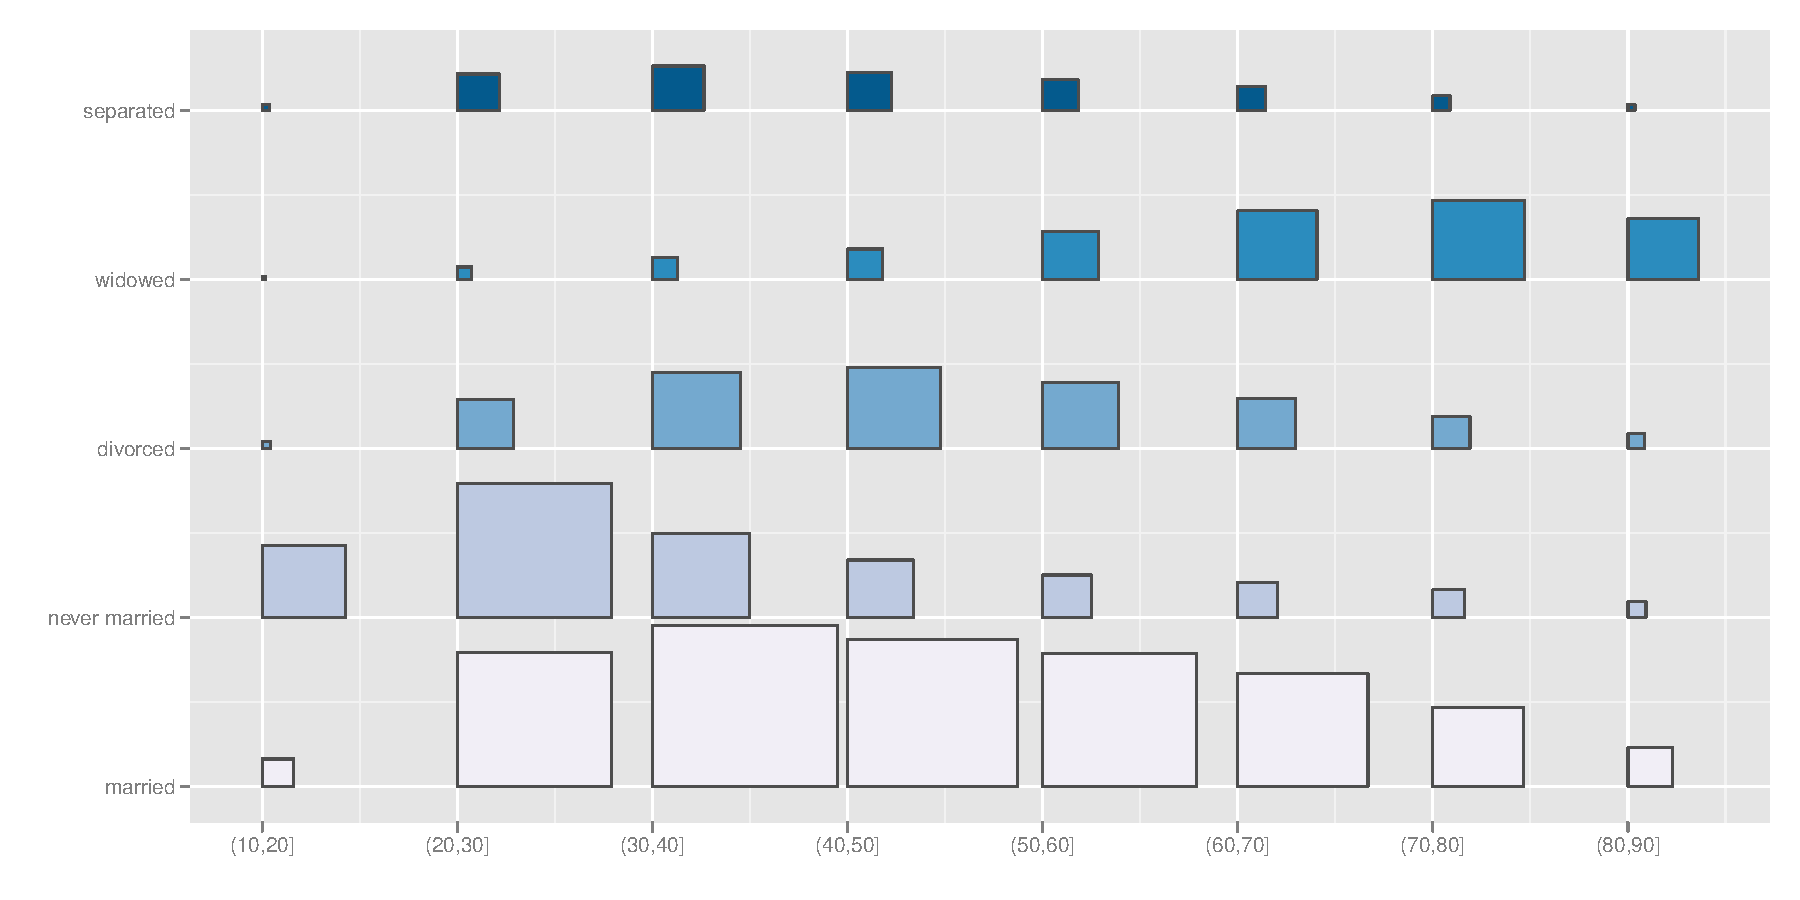
\includegraphics[width=0.9 \linewidth]{part-fluct}
    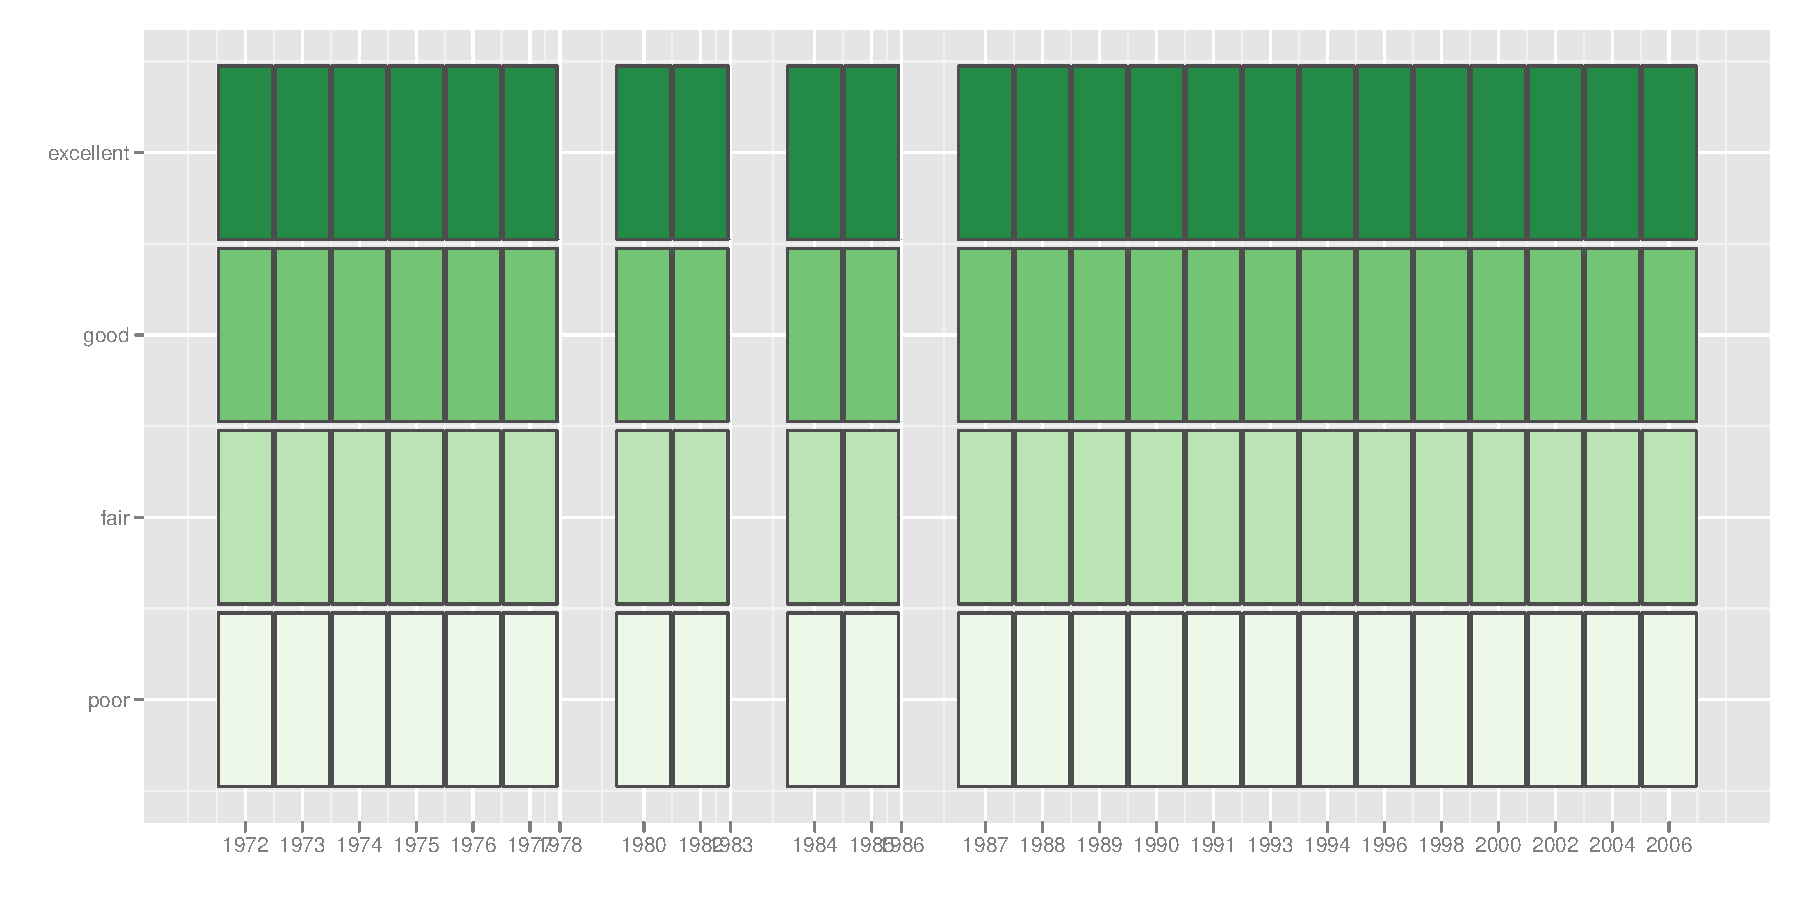
\includegraphics[width=0.9 \linewidth]{part-fluct-cond}
  \caption{(Left) A fluctuation diagram showing distribution of age (in decades) and marital status. (Right) Equal bin-size plot showing health status and survey year. Health status was not recorded for three years.}
  \label{fig:fluct}
\end{figure}

A special case of the fluct is the equal bin size plot \citep{hofmann:2000} which occurs when the two variables are jointly uniformly distributed, usually as a result of the conditioning described in the following section. The equal bin size plot is particularly useful as a way of visualising missing combinations. Figure~\ref{fig:fluct} illustrates these two types of graphics.

\section{Probability and plot products}
\label{sec:combination}

To construct plots of higher-dimensional data sets, we need a way to decompose them into 1d and 2d components. Some statistical vocabulary is useful. One way of describing the input data is as a {\bf probability mass function}, or {\sc pmf}. A {\sc pmf} is a function with n inputs, each indexing one dimension with an integer, and gives the probability of each combination of inputs. A {\sc pmf} has two restrictions: every value must be greater than or equal to zero, and all value must sum to one.  

\subsection{Products of probabilities}

Figure~\ref{fig:2d-table} shows three ways to represent the the 2d table of proportions of sex and happiness. The top table displays the {\bf joint distribution}, and allows us to answer questions of the form ``what proportion of all people are male and very happy?'' The middle two tables displays two {\bf conditional distributions}: the distribution of sex given happiness, and happiness given sex. These correspond to restriction the row or column sums to equal one, and support questions such as ``what proportion of pretty happy people are female?'' or ``what proportion of males are not too happy?''. Finally, the last table display the two {\bf marginal distributions} of sex and happiness. These allow us to answer questions like ``what proportion of respondents were male'' or ``what proportion of respondents were very happy?''.

\begin{figure}[ht]
  \begin{tabular}{rrr}
  \toprule
  & male & female \\ 
  \midrule
  not too happy & 0.05 & 0.07 \\ 
  pretty happy & 0.25 & 0.31 \\ 
  very happy & 0.14 & 0.18 \\ 
  \bottomrule
  \end{tabular}
  \\[1em]

  \begin{tabular}{rrr}
  \toprule
  & male & female \\
  \midrule
  not too happy & 0.43 & 0.57 \\
  pretty happy & 0.45 & 0.55 \\ 
  very happy & 0.43 & 0.57 \\
  \bottomrule
  \end{tabular}\hspace{1em}%
  \begin{tabular}{rrr}
  \toprule
  & male & female \\ 
  \midrule
  not too happy & 0.12 & 0.12 \\ 
  pretty happy & 0.57 & 0.55 \\ 
  very happy & 0.31 & 0.32 \\
  \bottomrule
  \end{tabular}
  \\[1em]

  \begin{tabular}{rrrr}
  \toprule
  & male & female & \\ 
  \midrule
  not too happy & & & 0.12 \\ 
  pretty happy & & & 0.56 \\ 
  very happy & & & 0.30 \\
  & 0.44 & 0.56 \\ 
  \bottomrule
  \end{tabular}

  \caption{The distribution of happiness and sex, displayed in three equivalent ways.  (Left) Joint distribution. Overall table sums to one. (Middle) Conditional distribution of sex given happiness and marginal distribution of happiness. (Right) Conditional distribution of happiness given sex and marginal distribution of sex.}
  \label{fig:2d-table}
\end{figure}

Formally, the conditional distribution is written as $f(x | y)$ and is equal to $f(x, y) / f(y)$. This definition illustrates that given a conditional distribution and a marginal distribution, we can always find the joint distribution: $f(x, y) = f(x | y) f(y)$ \footnotemark. This definition extends in a straightforward way to higher dimensions. For example, a 3d pmf can be written as the product of 2d and 1d conditional and marginal distributions as follows:

\footnotetext{Because the parameters of a pmf are identifying, statisticians often fail to distinguish the different functions.  To be precise, the above statement should be written: $f_{X, Y}(x, y) = f_{(X|Y=y)}(x | y) f_Y(y)$}

\begin{itemize}
  \setlength{\itemsep}{0em}
  \item $f(x, y, z) = f(z) f(x, y | z)$
  \item $f(x, y, z) = f(y, z) f(x | y, z) $
  \item $f(x, y, z) = f(z) f(y | z) f(x | y, z)$
\end{itemize}

This means that we can turn any high-dimensional {\sc pmf} into a product of low-dimensional conditional and marginal {\sc pmf}s products. It remains to find an graphical analog of this multiplication. 

\subsection{Area is a product of height and width}

We connect probability products to our rectangular primitives by noting that areas are also products, products of height and width. It's easiest to show this with a picture: Figure~\ref{fig:fact-simple} shows how our simple one primitives combine to get two familiar plots: the mosaic plot and the stacked bar chart. From left to right, we have plots of $f(happy)$, $f(happy | sex)$ and the product $f(happy, sex)$. The heights and widths of the rectangles are multiplied in the same way as the components of the {\sc pmf}.

\begin{figure}[htbp]
  \centering
  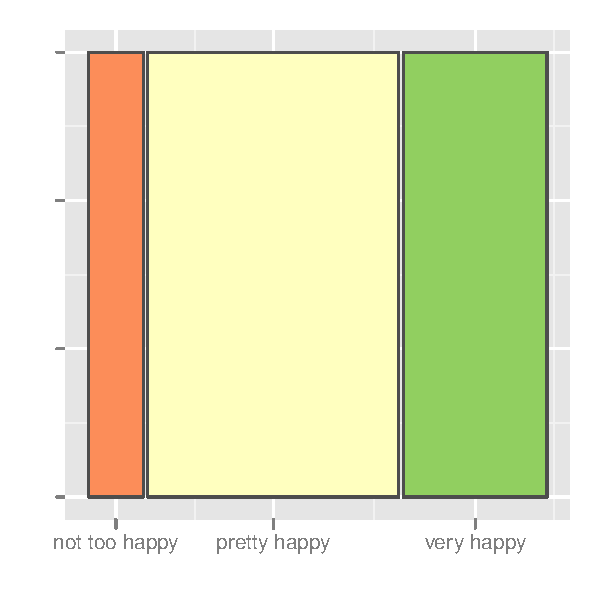
\includegraphics[width=0.3\linewidth]{fact-happy} $\times$ %
  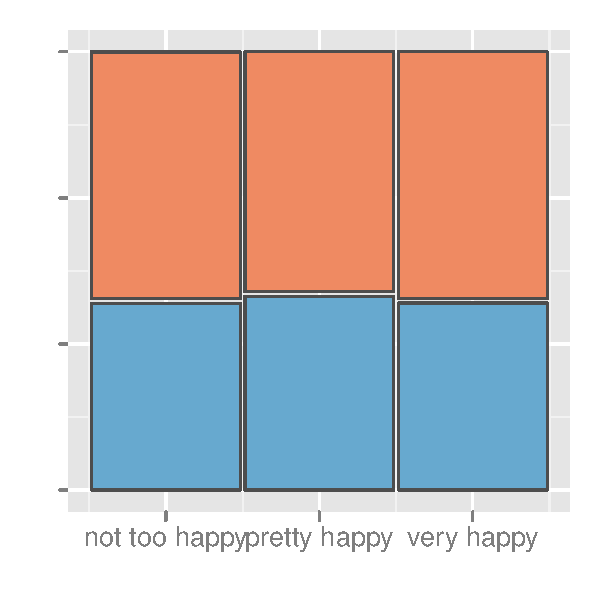
\includegraphics[width=0.3\linewidth]{fact-happy|sex} = %
  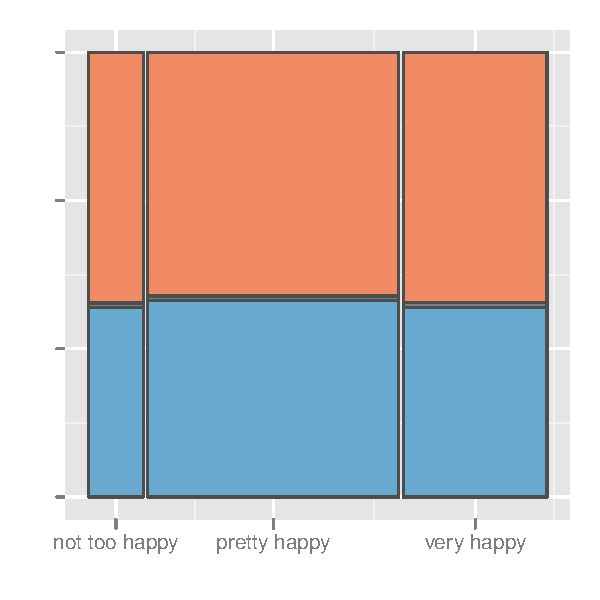
\includegraphics[width=0.3\linewidth]{fact-happy-sex}

  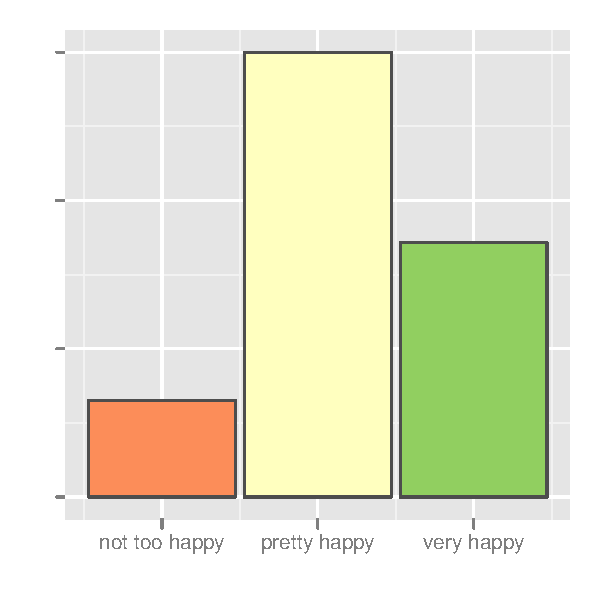
\includegraphics[width=0.3\linewidth]{fact-happy-2} $\times$ %
  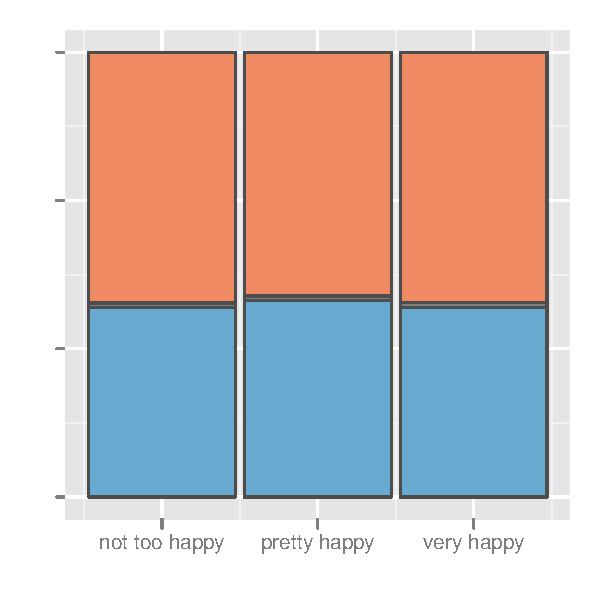
\includegraphics[width=0.3\linewidth]{fact-happy|sex-2} = %
  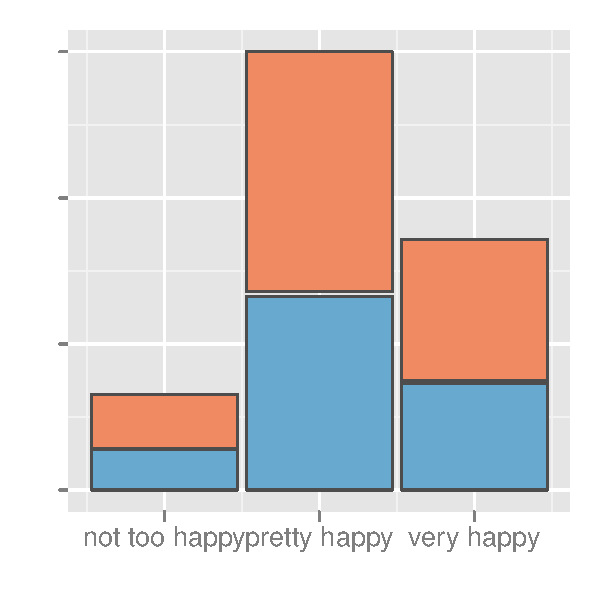
\includegraphics[width=0.3\linewidth]{fact-happy-sex-2}

  \caption{Plots of the distribution of happiness and sex (\key{male} male, \key{female} female).}
  \label{fig:fact-simple}
\end{figure}

Figure \ref{fig:recursive} shows the steps along by which a 3d dataset is displayed.  We first display $f(martial status)$, then $f(marital sex, sex) = f(sex | marital status) f(marital status)$, and finally $f(marital sex, sex, happiness) = f(happiness | sex, marital status) f(sex | marital status) f(marital status)$.

\begin{figure}[htbp]
  \centering
    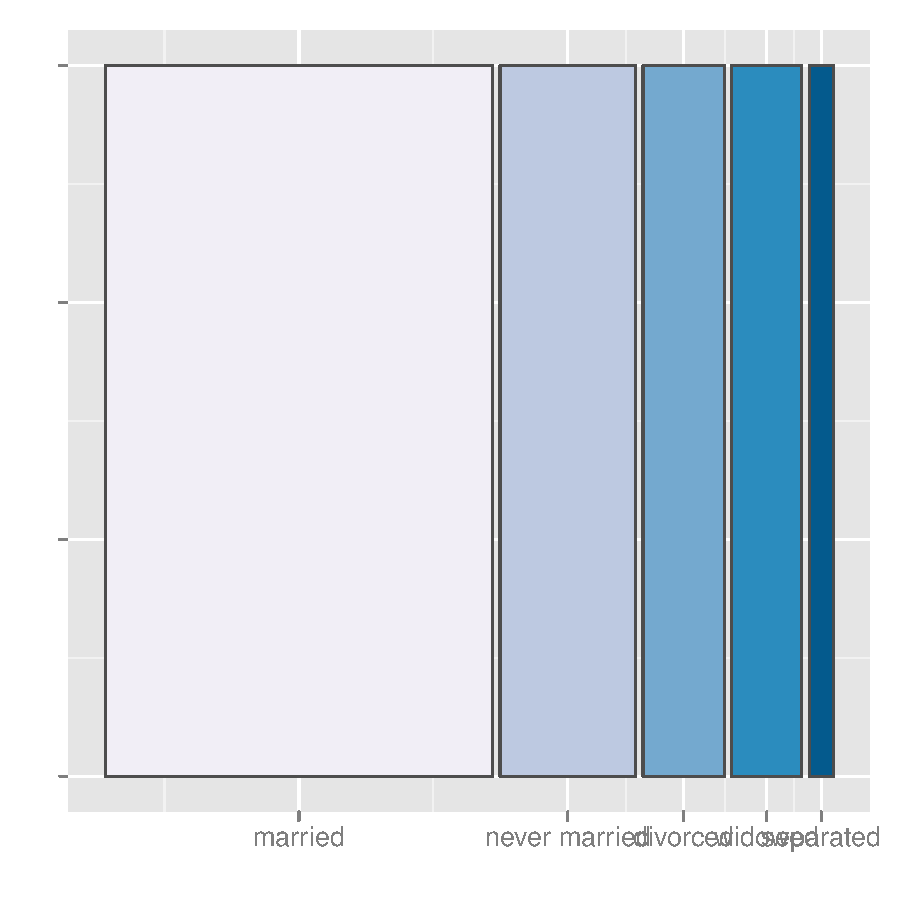
\includegraphics[width=0.33\linewidth]{part-comb-1}%
    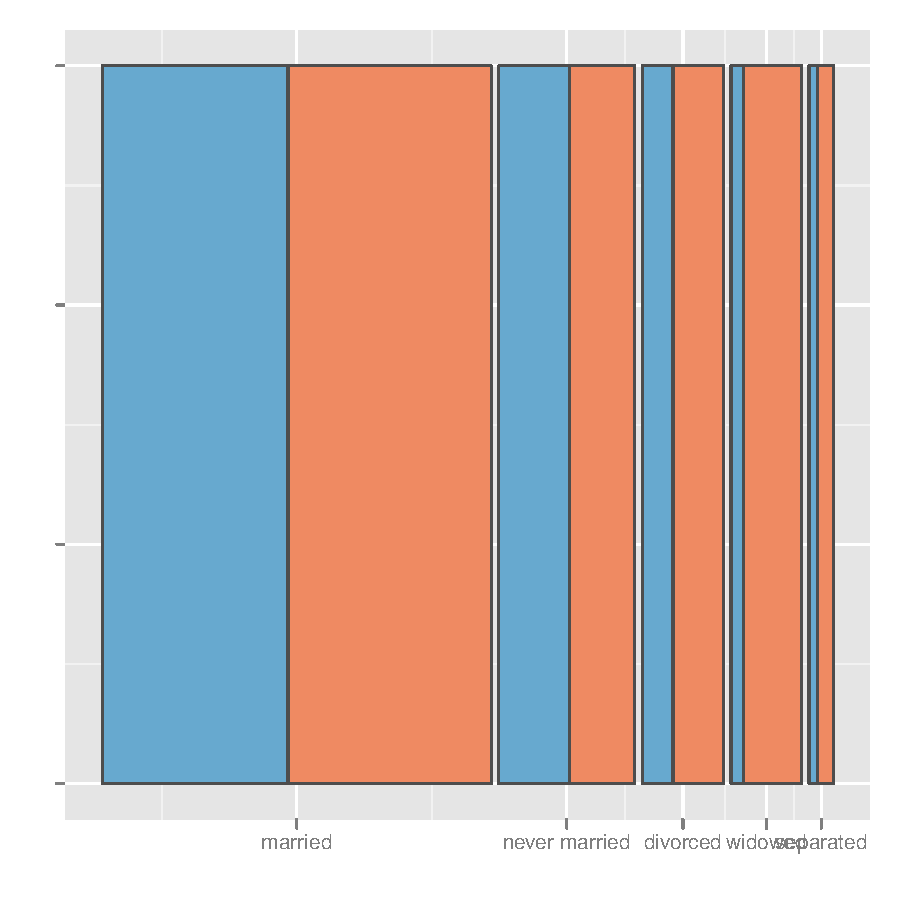
\includegraphics[width=0.33\linewidth]{part-comb-2}%
    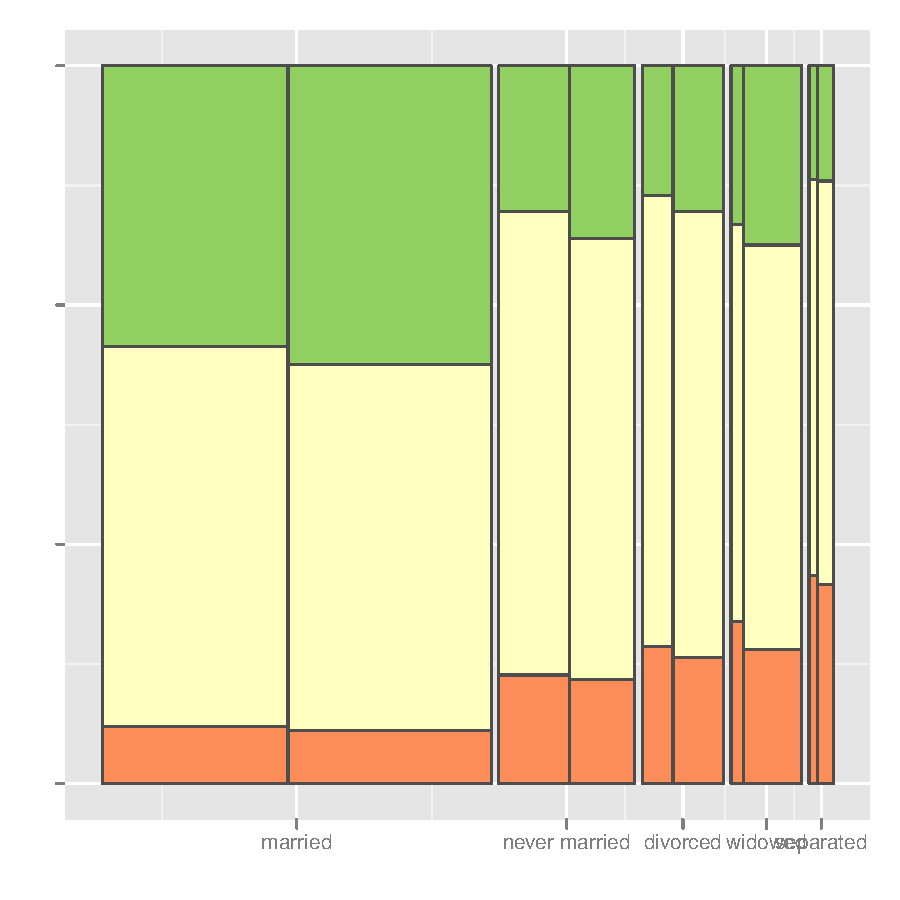
\includegraphics[width=0.33\linewidth]{part-comb-3}
  \caption{Conditional on marital status, are men or women happier?  This figure shows the construction of $f(happy, sex, marital)$ from (left to right) vspines by marital status, vspines by marital status and sex, and hspines by marital status, sex and happiness.  For all levels of marital status, men are slightly less happy.}
  \label{fig:recursive}
\end{figure}

% Note that while $f(x, y, z)$ and $f(z, y, x)$ represent the same pmf, the factorisation will be different because you will get different marginal tables.
% 
% Writing the full pmf is tedious, so we define an algebra based on the Wilkinson's modelling specification \citep{wilkinson:1973}:
% 
% \begin{itemize}
%   \setlength{\itemsep}{0em}
%   \item \verb|~ a| represents $f(a)$,
%   \item \verb|~ a + b| represents $f(a, b)$
%   \item \verb!~ a | b! represents $f(a | b)$
%   \item \verb!~ . | a! is a special case, $f(a) = \frac{1}{\#A}$.
% \end{itemize}
% 

% To visualise higher-dimensional pmfs, we recursively partition using the previously described primitives. That is, to display $f(x, y, z)$ we first create a partition based on $f(z)$ then partition each of those pieces based on $f(y | z)$ and again by $f(x | y, z)$.

Different combinations of partitions reveal different features of the data. Take for example, the distribution of age and marital status, as shown in Figure~\ref{fig:fluct}. Instead of visualisation the joint distribution with a fluct, we could focus on the conditional distribution of marital status, given age, or vice versa. Figure~\ref{fig:marital} shows two ways to do this. The left plot shows $f(marital, age)$ with a vspine nested in a hspine, and the right plot $f(age, marital)$ with a hbar nested in a vspine. These displays show the same data but are arranged in such a way to make different comparisons easier. The second plot, with bars nested inside spines, also illustrates important feature of non-space filling tilings: the relationship between proportion and area is only constant within a level. The bars are scaled to be as high as possible, without overflowing the bounding area.

\begin{figure}[htbp]
  \centering
    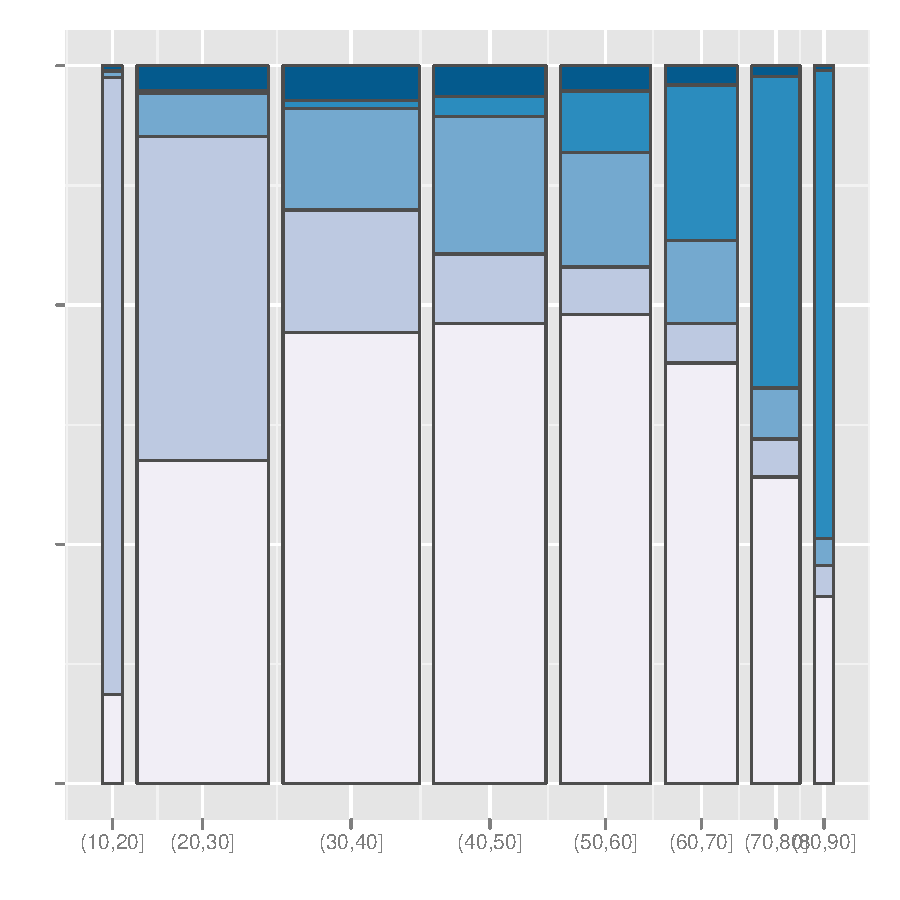
\includegraphics[width=0.5\linewidth]{part-marital-1}%
    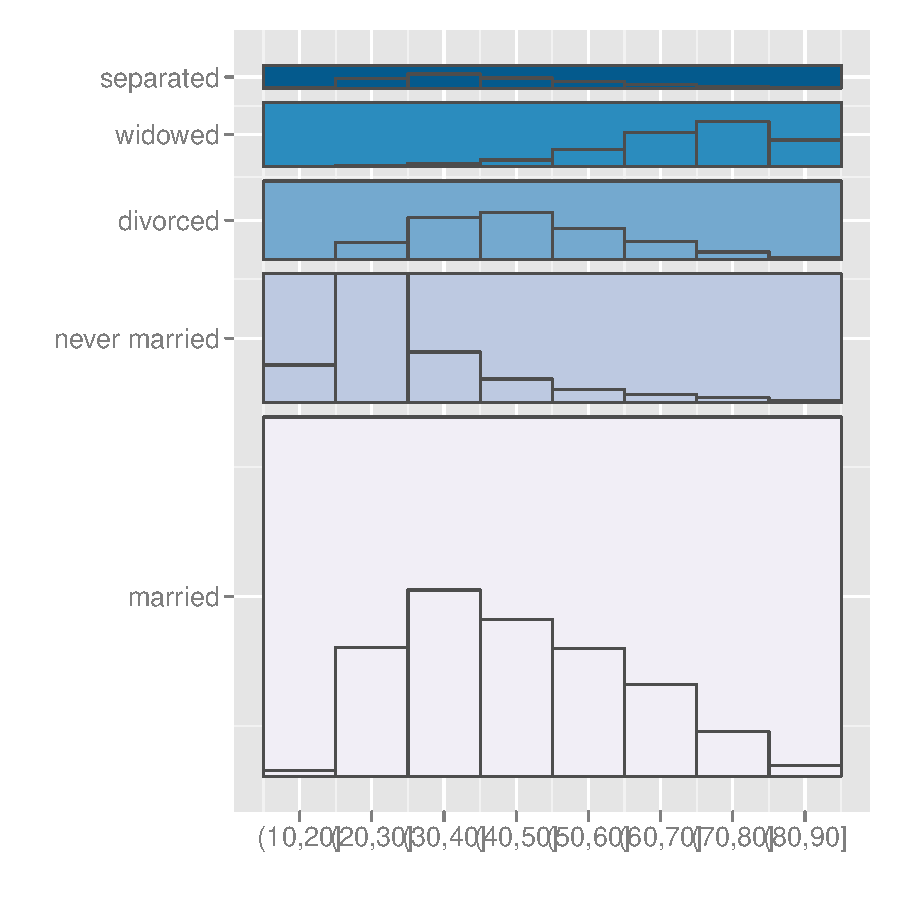
\includegraphics[width=0.5\linewidth]{part-marital-2}
  \caption{(Left) The joint distribution of marital status and age (in decades) partitioned by a vspine and hspine.  (Right) The joint distribution of age and marital status partitioned by a vspine and hbar.}
  \label{fig:marital}
\end{figure}

Conditioning is also an important tool by itself, because it allows one to remove relationships that are well-known or uninteresting. Figure~\ref{fig:part-cond} uses a fluct and a vspine to explore the relationship between happiness, health and financial status. The left plot displays raw proportions, showing that most people are in good health and average financial standing. However, it is difficult to see how happiness varies within these conditions because the perceptual task is comparing areas. Conditioning on financial status and health produces the plot on the right (an equal bin size plot) and makes it easier to see the conditional distribution of happiness given sex and health, because the perceptual task is simpler.  Depending on the comparison we are most interested in, we can make it easier to compare across wealth for fixed health, or health for fixed wealth. 

For this data, for a fixed income level, happiness always increases as health increases. The same is not true for fixed health: those with poor or fair health are actually less happy if they are far above average, compared to just above average.

\begin{figure*}[htbp]
  \centering
    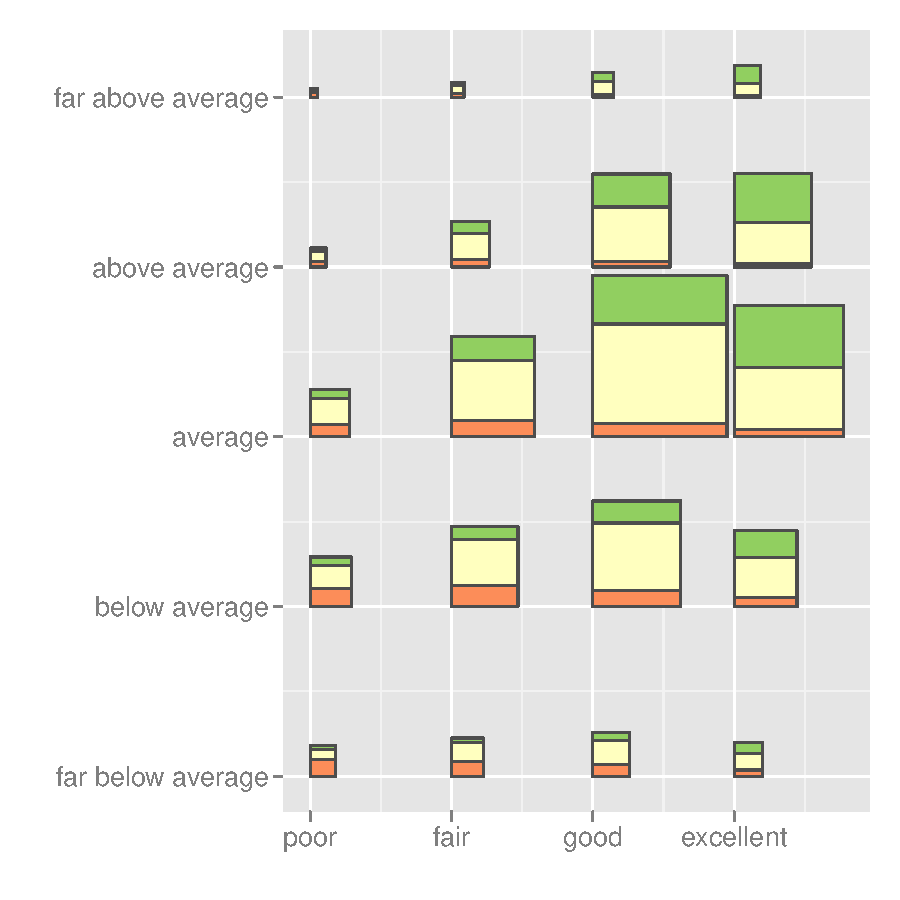
\includegraphics[width=0.33\linewidth]{part-fluctuation}%
    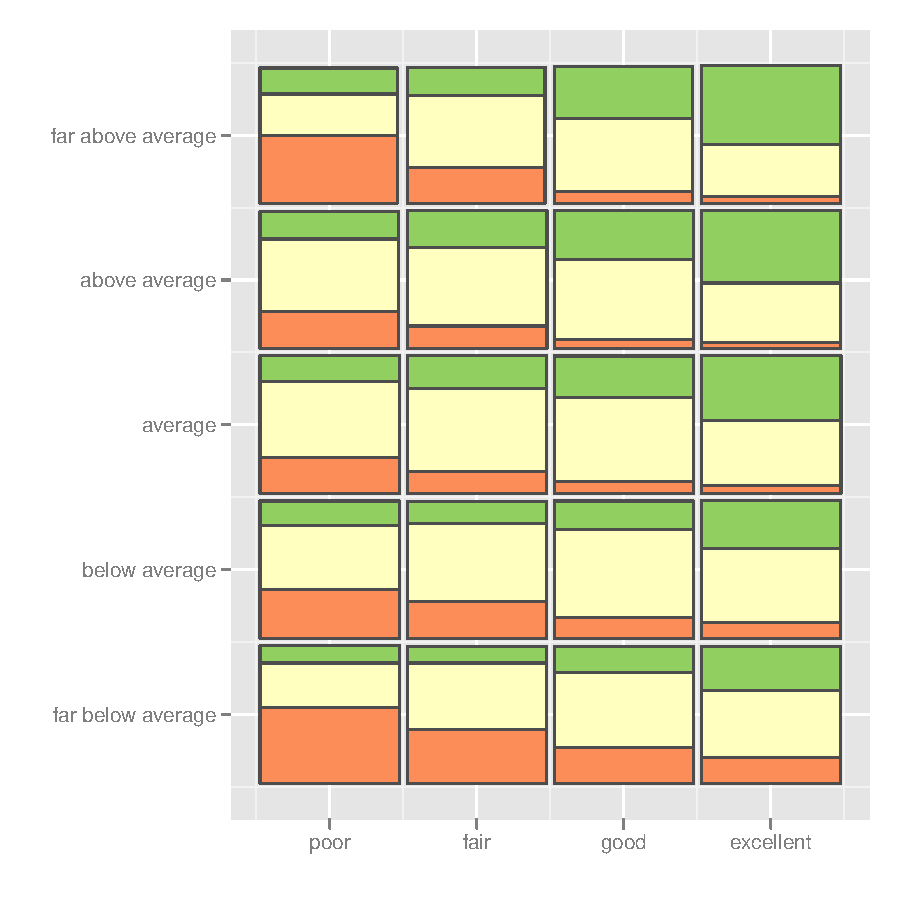
\includegraphics[width=0.33\linewidth]{part-equal-area}%
    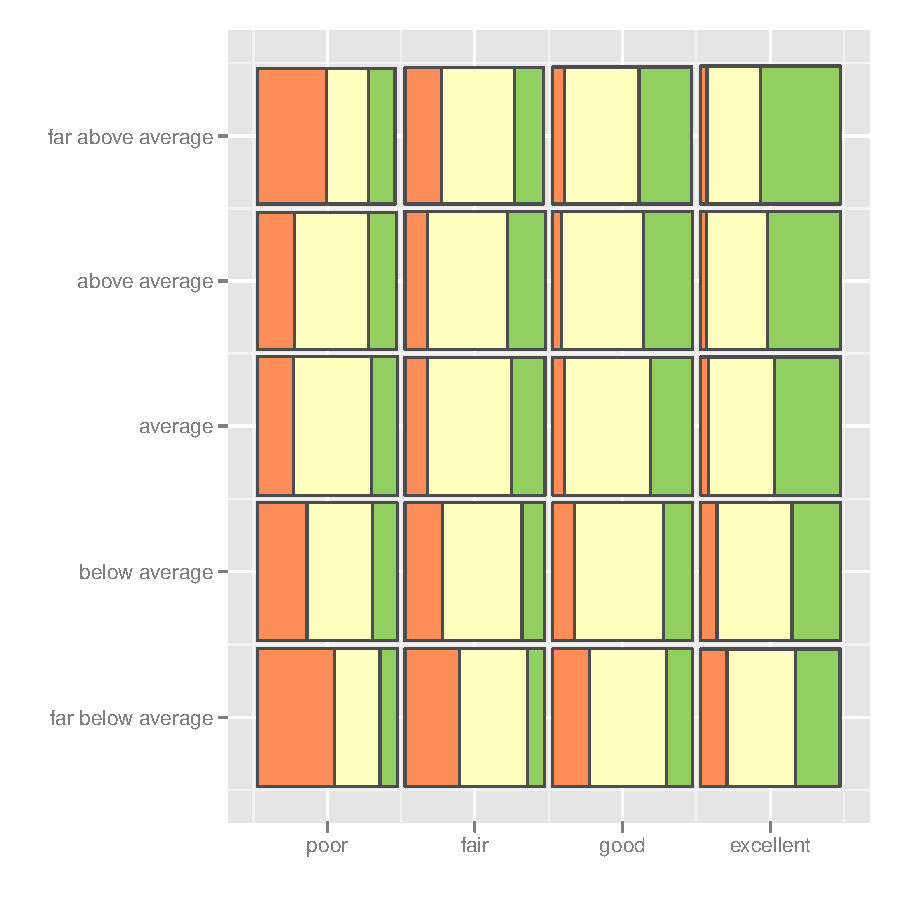
\includegraphics[width=0.33\linewidth]{part-equal-area-2}
  \caption{(Left) $f(happy, health, finrela) = f(happy | health, finrela) \times f(health, finrela)  $, partitioned with a vspine and fluct.  (Middle) $f(happy | health, finrela)$. We can no longer see the joint distribution of health and financial status, but it is much easier to see the conditional distribution of happiness. Healthier and richer people are happier: maybe money does buy happiness? (Right) $f(happy | health, finrela)$ partitioned with a fluct and {\bf h}spine. (\key{not-too-happy} Not too happy, \key{pretty-happy} pretty happy, \key{very-happy} very happy)}
  \label{fig:part-cond}
\end{figure*}

\section{Existing plot types}
\label{sec:existing}

Many existing plots fall into this framework. The primitives already have their own names:

\begin{itemize}
  \setlength{\itemsep}{0em}
  \item {\bf Bar chart} (1d). 1 hbar.
  \item {\bf Column chart} (1d). 1 vbar.
  \item {\bf Spineplot} (1d). 1 spine.
  \item {\bf Fluctuation} diagram (2d): 1 fluct.
\end{itemize}

\noindent And many more plots correspond to higher order combinations:

\begin{itemize}
  \setlength{\itemsep}{0em}
  
  \item {\bf Stacked} bar chart (2d). 1 hbar and 1 vspine.

  \item {\bf Nested} bar chart \citep{peltier:2009} (2d).  2 hbars. 

  \item {\bf Equal bin size} \citep{hofmann:2000} plot (3d): fluct and vspine, conditioned on the first two variables.

  \item {\bf Mosaic} plot \citep{hartigan:1981,friendly:1994,hofmann:2003} (nd). Alternating hspines and vspines. 

  \item {\bf Double-decker} plot \citep{hofmann:2001} (nd). $n-1$ hspines and 1 vspine. 

  \item {\bf Treemap} \citep{shneiderman:1992} (nd): n spines.

  \item {\bf Squarified treemap} \citep{bruls:1999} (nd): n tiles. 

  \item {\bf Generalised treemaps} \citep{vliegen:2006} (nd): any plot ending with a tile.

\end{itemize}

Trellis graphics \citep{becker:1996}, also known as lattice, facetted and conditioned graphics, are another related display. They use categorical variables to generate multiple panels, each containing a plot of the subset of the data. Trellised area plots also fall into our framework and can be created by conditioning on the trellising variables.


\section{Variations and extensions}
\label{sec:variations}

On top of this basic framework, it is useful to consider a few variations and extensions. Instead of count of discrete levels, we can plot weighted data or continuous data, or we can relax the display constraints to allow displays where area is not proportional to weight, partitions are non-disjoint or non-rectangular.

\subsection{Weighting}
\label{sub:weighting}

We have assumed that the proportions represent counts, but without loss of generality, we can use any set of non-negative, additive weights. For example, in the happy dataset, the {\sf wtssall} variable gives analytic survey weights. These are use to account for oversampling of black respondents in certain years, and to reduce the effect of non-response by other demographics. Figure~\ref{fig:weighting} shows the difference between the weighted and unweighted distributions of age and sex. The distribution is subtly different, and suggests that we don't need to worry about weights for this plot. In other datasets, weights can be useful to move from numbers of counties to numbers of people, or to areas, or to other relevant quantities. Some examples of weighted data graphics can be found in \citep{unwin:1998,unwin:2003aa,unwin:2006}.

\begin{figure}[htbp]
  \centering
    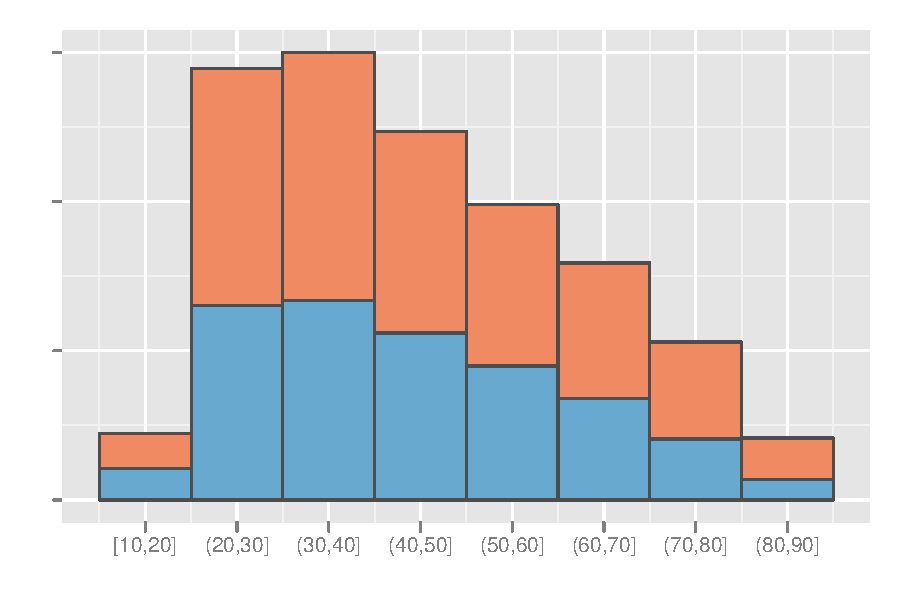
\includegraphics[width=0.5\linewidth]{wt-count}%
    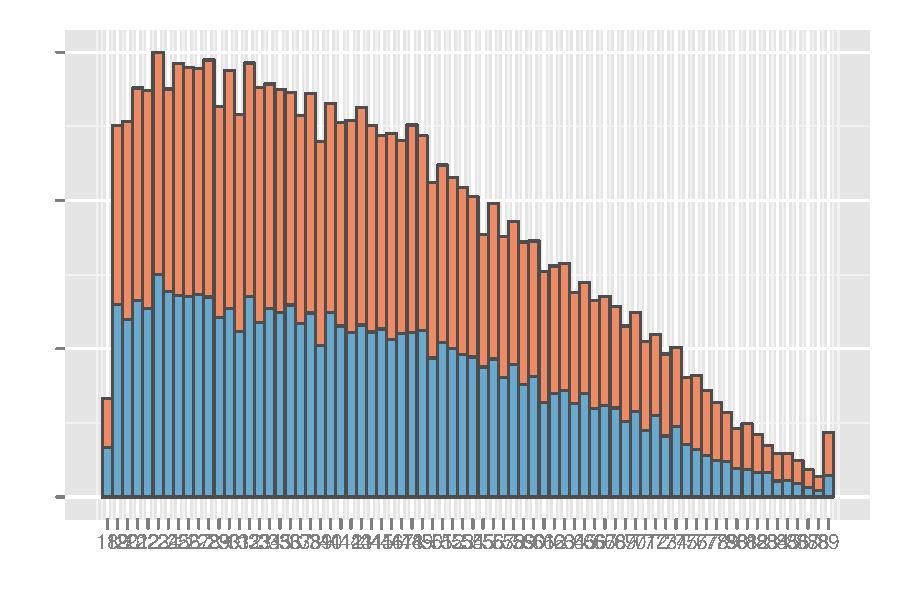
\includegraphics[width=0.5\linewidth]{wt-wtssall}%
  \caption{Joint distribution of age and sex (\key{male} male, \key{female} female). (Left) counts and (right) probability weights.}
  \label{fig:weighting}
\end{figure}

\subsection{Continuous data}
\label{sub:continuous_data}

The framework can be trivially extended to work with continuous data: just first bin continuous variables. There are many different to ways to create intervals for continuous data, but two are most important \citep{denby:2009}: intervals of equal width, and intervals containing equal numbers of points. This extension allows the product plot framework to also describe {\bf histograms} and {\bf spinograms} \citep{hummel:1996}, continuous analogues of the bar and charts. A long standing tradition is that no gaps are displayed between adjacent rectangles when used for continuous data. Two examples are shown in Figure \ref{fig:cont-examples}.

\begin{figure}[htbp]
  \centering
  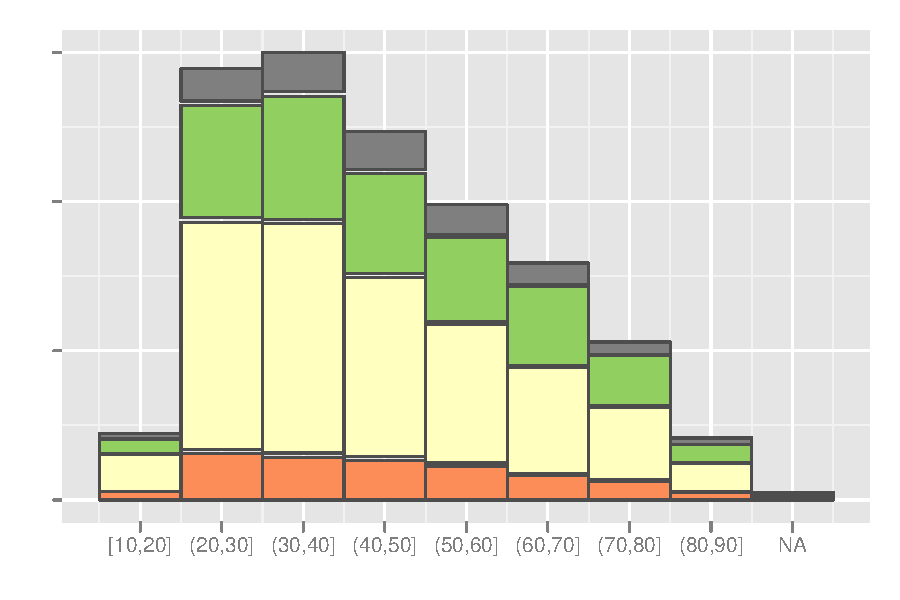
\includegraphics[width=0.5\linewidth]{cont-hbar}%
  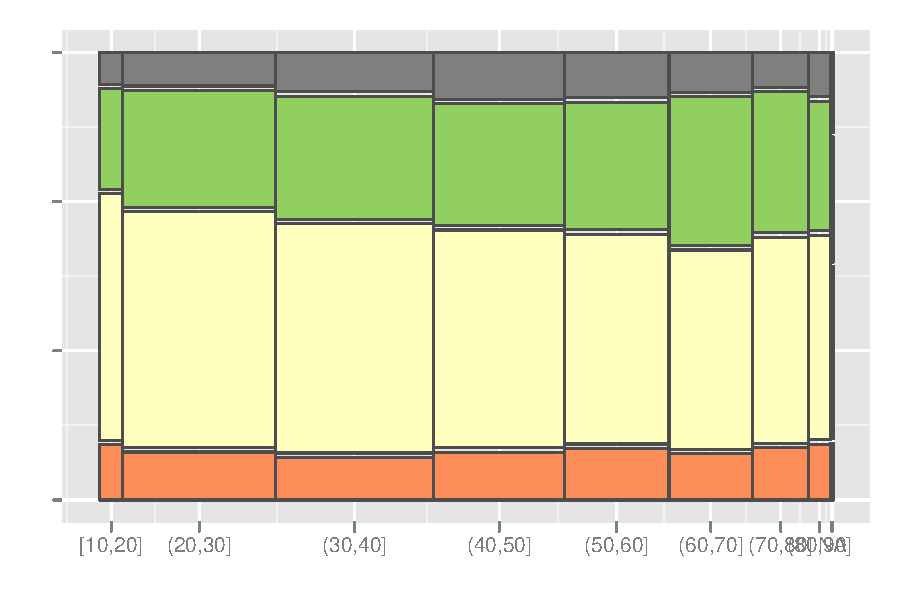
\includegraphics[width=0.5\linewidth]{cont-hspine}
  
  \caption{The distribution of happyness with age. (Left) hbar + vspine: an extension of the histogram. (Right) hspine + vspine: an extesion of the spinogram.}
  \label{fig:cont-examples}
\end{figure}

With one more extension, displaying the final probability with colour, not area, this allows us to describe {\bf dimensional stacking} \citep{leblanc:1990} as a plot of conditioned, binned continuous data, with proportion shown with colour. 

\subsection{Area not proportional to weight}

It can be useful to violate the constraint that area should be proportional to weight to distinguish between zeros and very small values. A zero weight should have zero area, but giving it positive area can be useful that so you can actually see it! In general, it's useful to constrain all areas to be above a certain minimal perceptible size. Areas which are constrained in such a way should have a visual flag (such as a difference colour) so ensure that the reader knows that the relationship between area and value has been violated. This type of non-linear mapping has been implemented in {\sc manet} \citep{unwin:1996} and hierarchical pixel bar charts \citep{keim:2002}.

On the other end of the spectrum, it can be useful to constrain put a cap on the size of largest values to get censored zooming \citetext{Antony Unwin, priv. comm.}. Controlling this cap makes it possible to focus on the smallest values.

Other non-linear transformations may also be useful. For example, we could display the square root of the weights, to stabilise the variance of the areas. Tukey applied this technique to histograms to create rootograms \citep{wainer:1974,tukey:1977}: histograms where the y-axis has a square root scale.

\subsection{Non-disjoint partitions}

The cascaded treemaps of \citet{lu:2008} is an idea that illustrates how the violation of containment can be productive. In the {\bf cascaded treemap}, each level is slightly offset from the one above to create a pseudo-3d perspective. This makes it easier to see all the levels of the hierarchy, not just the lowest level. Figure~\ref{fig:cascade} shows an example of how cascading can help illuminate the structure of a complex mosaic plot.

\begin{figure}[htbp]
  \centering
    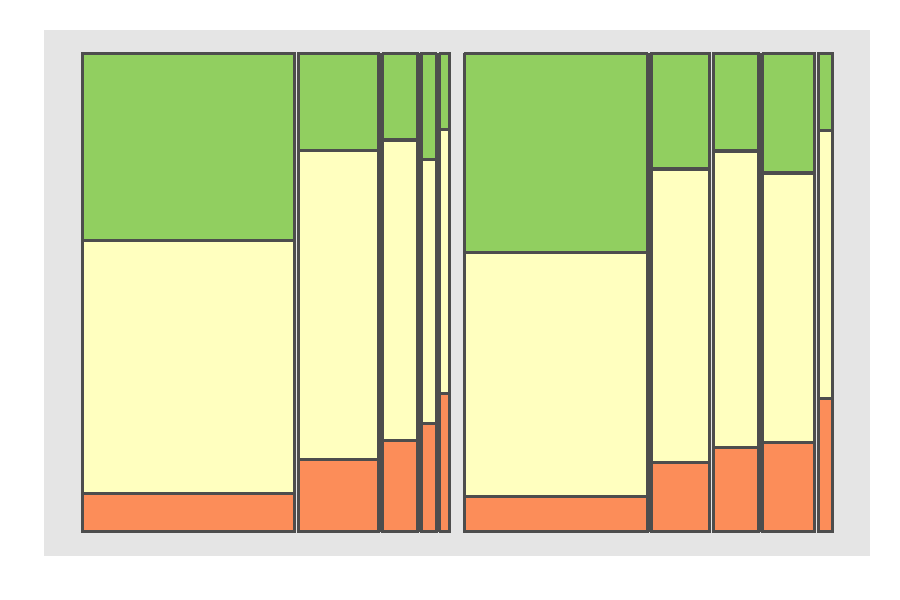
\includegraphics[width=0.5\linewidth]{sex-marital-happy}%
    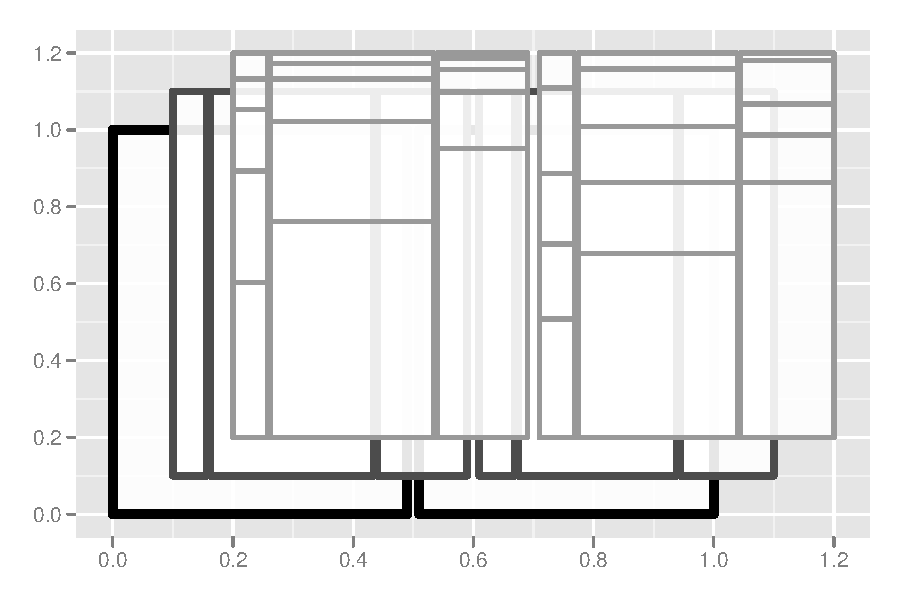
\includegraphics[width=0.5\linewidth]{cascade}
  \caption{A mosaic plot of happiness by martial status and sex. (Left) Coloured by happiness (\key{not-too-happy} Not too happy, \key{pretty-happy} pretty happy, \key{very-happy} very happy).  (Right) A cascaded view helps show how the plot is built up.}
  \label{fig:cascade}
\end{figure}

\subsection{Non-rectangular partitions}

A pie chart is a popular method of displaying proportions, but it is not a rectangular partition and so does not seem to fall in the framework of this paper. However, there is a simple relationship between product plots and pie charts: an pie chart is an hspine drawn in polar coordinates with the x coordinate mapped to angle and the y coordinate to radius. 

Many other circular displays turn out to be special cases of product plots drawn in polar coordinates \citep{draper:2009}. Generally, the y axis (mapped to radius) must be square-root transformed to ensure that that counts stay proportional to areas. Stasko's radial displays \citep{stasko:2000} and fan-lenses \citep{lou:2007} deliberately do not do this in order to emphasise the outer levels.

We have identified the following radial plots as polar transformations of product plots:

\begin{itemize}
  \setlength{\itemsep}{0em}
  
  \item {\bf Wind rose} (aka sector graphic) \citep{lalanne:1843} and {\bf fourfold displays} \citep{friendly:1995} (2d): 1 hbar, and 1 vspine. Nightingales's coxcomb \citep{nightingale:1857} is very similar, but the slices overlap and so violate the constraint of disjoint area.

  \item {\bf Concentric pie chart} (aka bullseye chart) (1d): 1 hspine.

  \item {\bf Doughnut plot} (2d): 1 hspine, and 1 vspine.

  \item {\bf Racetrack plot} (aka circular bar chart) (1d): 1 vbar.

  \item {\bf Infoslices} \citep{andrews:1998} (nd): n vbars. But they only use half of the polar plane, and are specialised for highly nested data.

\end{itemize}

\noindent Eight polar variants are displayed in Figure~\ref{fig:polar}. Many of these are familiar and already have names. They are all of dubious utility because of the increased difficulty when comparing non-rectangular areas.

\begin{figure}[htbp]
  \centering
    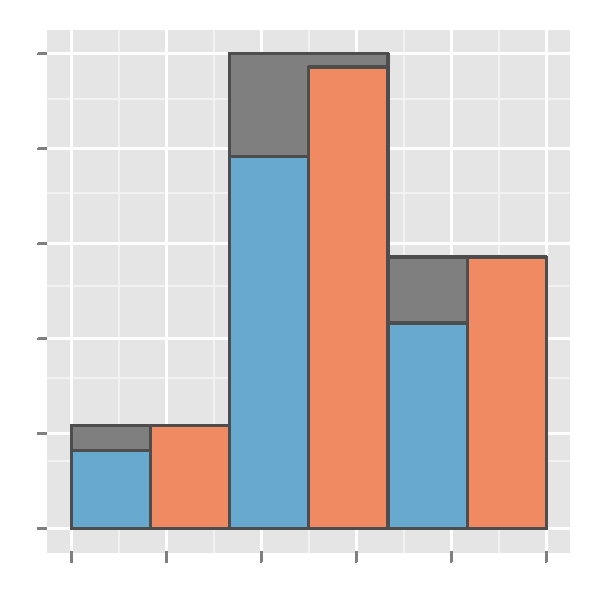
\includegraphics[width=0.25\linewidth]{hb-vb-cartesian}%
    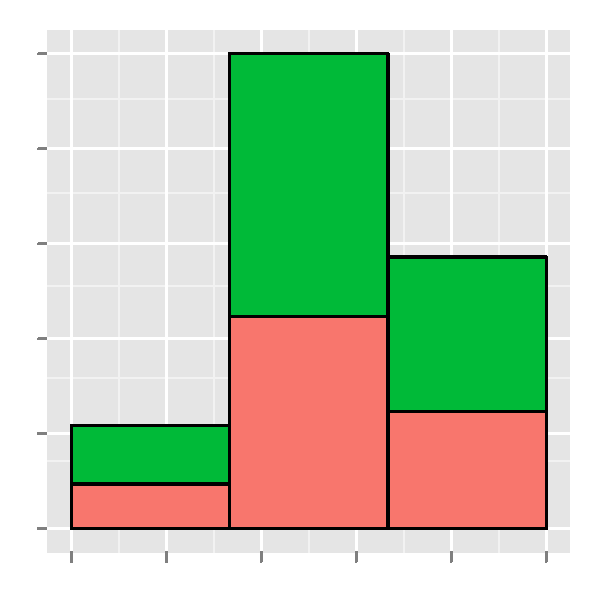
\includegraphics[width=0.25\linewidth]{hb-vs-cartesian}%
    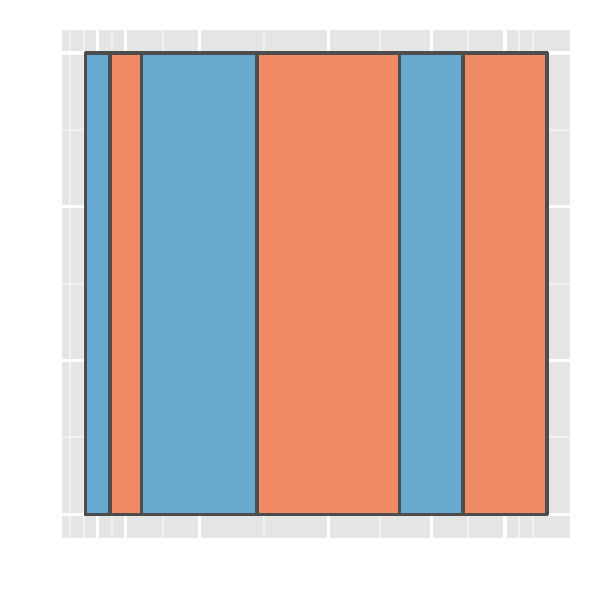
\includegraphics[width=0.25\linewidth]{hs-hs-cartesian}%
    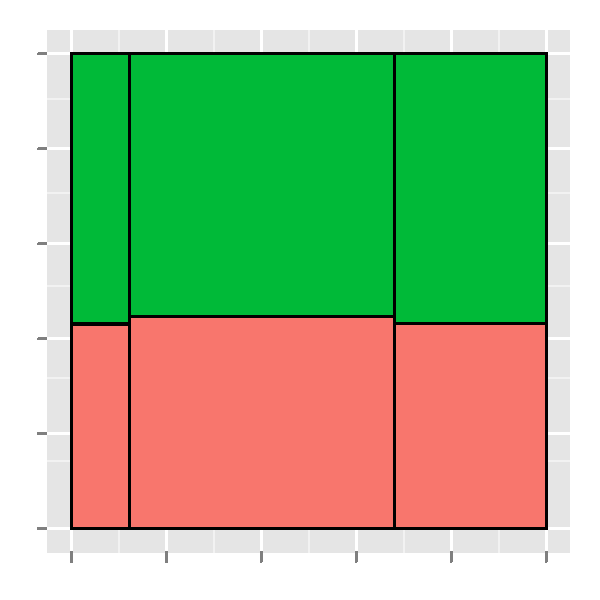
\includegraphics[width=0.25\linewidth]{hs-vs-cartesian}

    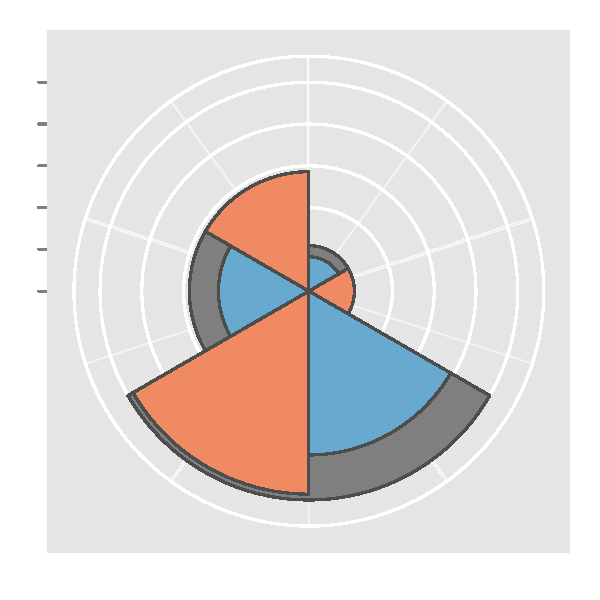
\includegraphics[width=0.25\linewidth]{hb-vb-polar}%
    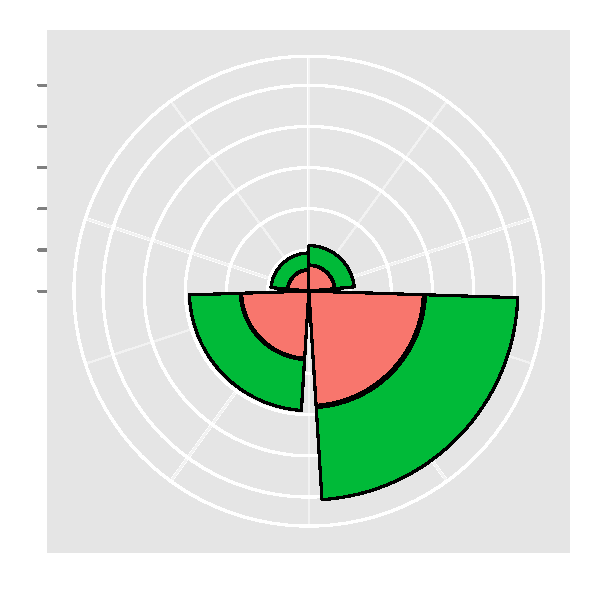
\includegraphics[width=0.25\linewidth]{hb-vs-polar}%
    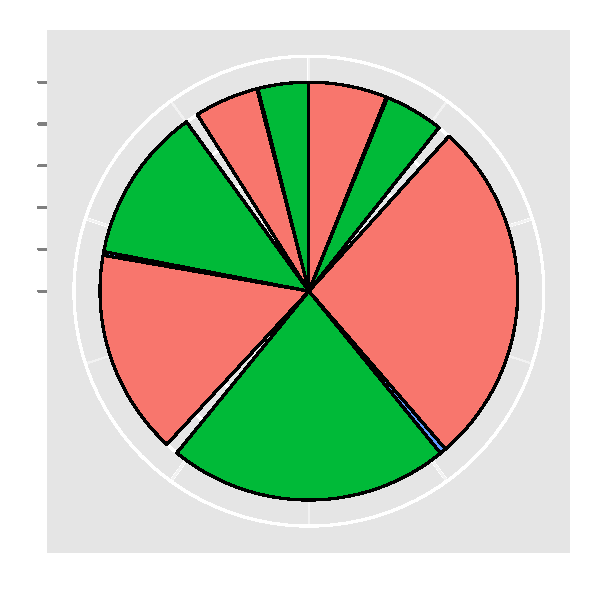
\includegraphics[width=0.25\linewidth]{hs-hs-polar}%
    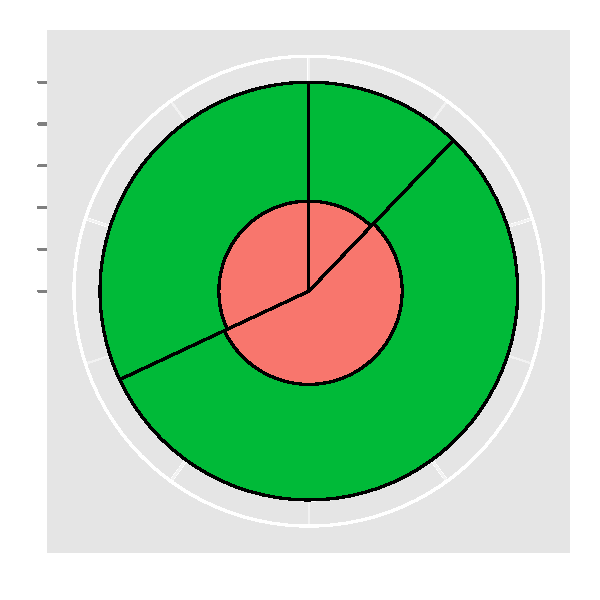
\includegraphics[width=0.25\linewidth]{hs-vs-polar}

    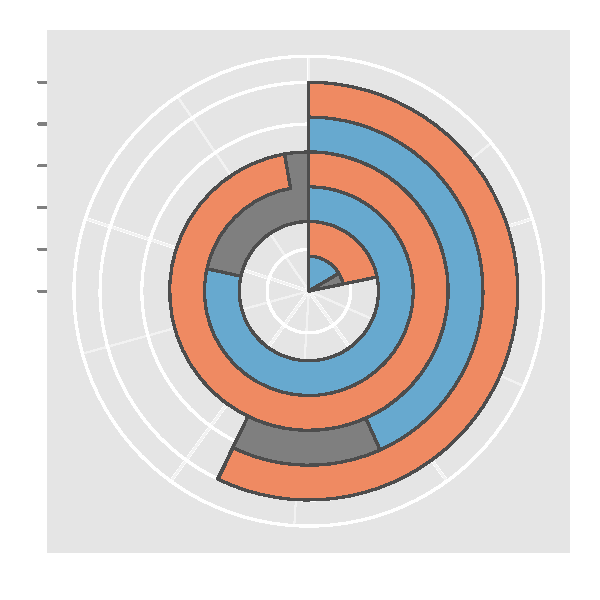
\includegraphics[width=0.25\linewidth]{hb-vb-polar-2}%
    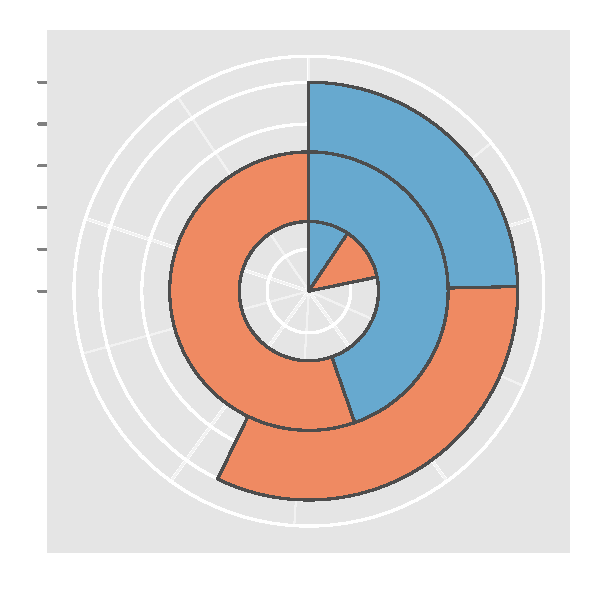
\includegraphics[width=0.25\linewidth]{hb-vs-polar-2}%
    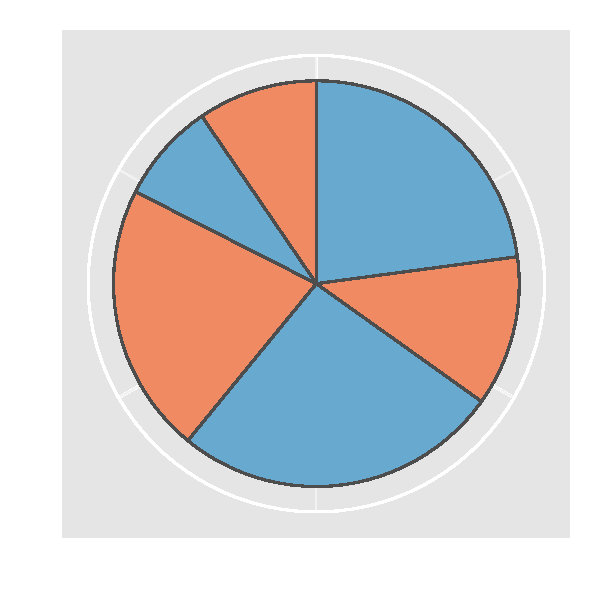
\includegraphics[width=0.25\linewidth]{hs-hs-polar-2}%
    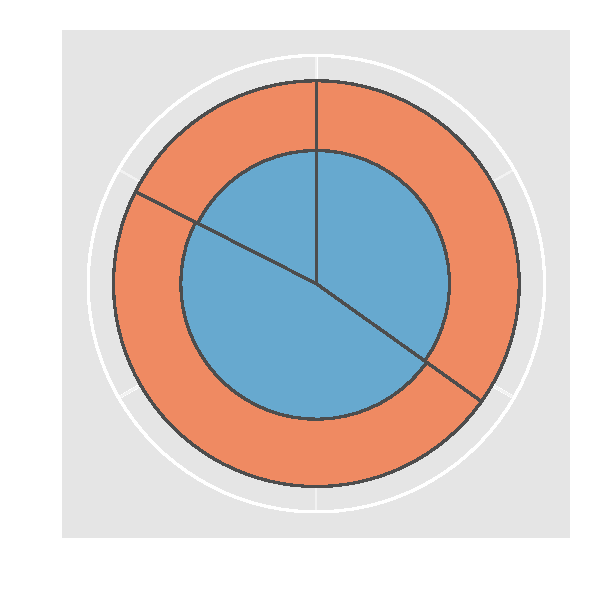
\includegraphics[width=0.25\linewidth]{hs-vs-polar-2}

  \caption{(Top) Area graphics in Cartesian coordinates. (Mid) Area graphics in polar coordinates. From left to right: hbar + hbar, vspline + hbar, hspine + hspine, hspine + vspine. (Bottom) Product graphics rotated 90 degrees before being converted to polar coordinates: vbar + vbar, hspline + vbar, vspine + vspine, vspine + hspine. (\key{male} male, \key{female} female)}

  \label{fig:polar}
\end{figure}

A number of non-rectangular treemaps have been proposed, such as circular treemaps \citep{wetzel:2008}, space-filling curves \citep{wattenberg:2005} and voronoi treemaps \citep{balzer:2005}. The perceptual task associated with these visualisations is the comparison of the area of arbitrary polygons, which is much more difficult than comparing the area of rectangles \citep{cleveland:1986}. This makes these approaches attractive rather than useful.

% \section{Aesthetics}
% \label{sec:aesthetics}
% 
% \subsection{Labelling} 
% \label{sub:labelling}
% 
% \subsection{Offsets}
% \label{sub:offsets}
% 
% 
% \section{Interaction}
% \label{sec:interaction}



\section{Conclusions}

This framework leads to a combinatorial explosion of possibilities. A 4d pmf, f(a, b, c, d) can be factorised in five different ways:

\begin{itemize}
  \item $f(a, b, c, d) = f(a | b, c, d) f(b | c, d) f(c, d)$
  \item $f(a, b, c, d) = f(a | b, c, d) f(b | c, d) f(c | d) f(d)$
  \item $f(a, b, c, d) = f(a | b, c, d) f(b, c | d) f(d)$
  \item $f(a, b, c, d) = f(a, b | c, d) f(c, d)$
  \item $f(a, b, c, d) = f(a, b | c, d) f(c | d) f(d)$
\end{itemize}

\noindent There are 24 possible ways of ordering the variables in the pdf, and each 1d pmf can be displayed in five different ways. For a 4d problem this gives $5 * 24 * (5^3 + 5^4 + 5^2 + 1 + 5^2) = 96,120$ plots! In future work, we hope to connect product plots to statistical models to help guide the choice of appropriate graphic.

We are also interested in exploring the automated construction of a graphic to answer specific questions, and for given a plot, suggesting which type of questions it is most suitable to answer.

% \acknowledgments{ The authors wish to thank Robert Kosara for helpful discussion. This work was partly supported by the National Science Foundation grant DMS0706949. Graphics produced with ggplot2 \citep{me:ggplot2}.}

% bibtool -x prodplots-infovis -o references.bib
\bibliographystyle{ieeetr}
\bibliography{references}

\end{document}
